\documentclass[11pt]{article}

\usepackage{graphicx}
\usepackage{amsmath}
\usepackage{siunitx}
\usepackage[a4paper, total={6in, 10.5in}]{geometry}
\usepackage{titling}
\usepackage{listings}
\usepackage{float}
\usepackage{subcaption}
\usepackage{pdfpages}
\usepackage{bbm}
\usepackage{amsfonts}

\graphicspath{{figures/}}
\title{\vspace{-2cm}4F13 Coursework 2 - Probabilistic Ranking}
\preauthor{}
\author{}
\postauthor{}
\date{November 2024}

\setlength{\belowcaptionskip}{-10pt}

\begin{document}

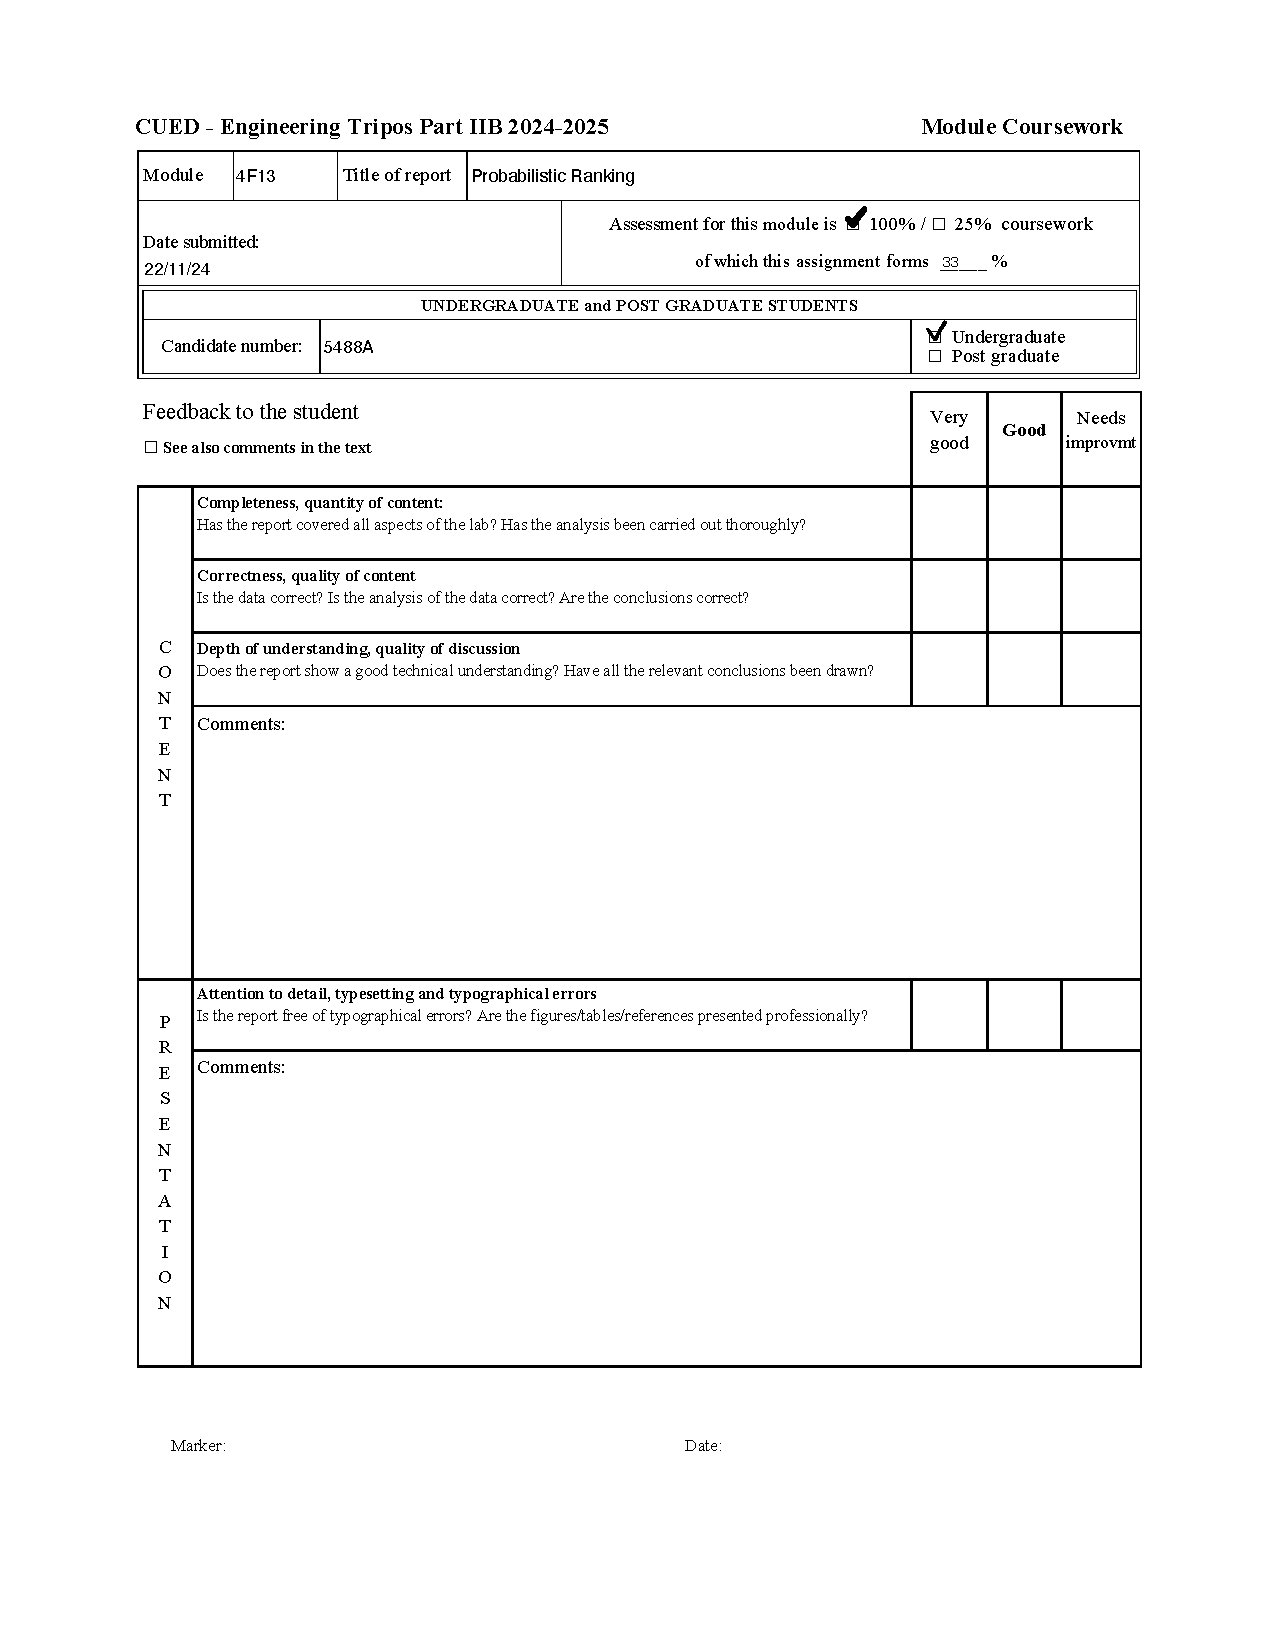
\includepdf[pages={1}]{coversheet}

\setcounter{page}{1}

\maketitle

\section{Task A}

Figure \ref{fig:A_skill_samples} shows samples of the skills at each Gibbs iteration for 3 players. We see that at each iteration the sampled skill of each player appears random but perhaps not independent of the previous iteration. This is expected from an MCMC method like Gibbs sampling and shown better by the auto covariance plot in Figure \ref{fig:A_auto_covariance}. 

\begin{figure}[h]
    \centering
    \includegraphics[width=\linewidth]{A/skill_samples} 
    \caption{Samples of the skill of 3 players at each Gibbs iteration.}
    \label{fig:A_skill_samples}
\end{figure}

If the samples at each iteration were independent we would expect the auto covariance to be zero for all non zero lags. However, we notice that the auto covariance only converges to zero for all players for lags greater than 10. This indicates that if we kept only every 10th sample they would be independent, this is the logic behind thinning. We do not need to employ thinning techniques here as we are not running into memory issues but it is a useful tool for large datasets.

\begin{figure}[h]
    \centering
    \includegraphics[width=\linewidth]{A/auto_covariance} 
    \caption{Skill sample auto covariance for all players}
    \label{fig:A_auto_covariance}
\end{figure}

The convergence of the skill population is shown in Figure \ref{fig:A_convergence}. We see that there is no clear burn in time for the population mean but the standard deviation takes about 5 iterations to enter the high probability region. This makes sense from our auto covariance analysis as we concluded samples 10 iterations apart are roughly independent so the burn in time should be no more than 10 iterations. For any further analysis we will discard the first 100 Gibbs iterations as burn in time to be sure.

\begin{figure}[h]
    \centering
    \includegraphics[width=\linewidth]{A/convergence} 
    \caption{Skill populations mean and standard deviation with Gibbs iteration.}
    \label{fig:A_convergence}
\end{figure}

To estimate how many iterations we need to run the Gibbs sampler to get skill estimates within a certain tolerance we can analyse the variance of our Monte Carlo skill estimates. Equation \ref{eq:gibbs_skill_variance} calculates the variance of the Gibbs skill estimate, $\bar{w_i}$, for player $i$ after $N$ iterations. The variance depends on the sum of the auto covariance, $\frac{\sigma_i^{(t)2}}{\text{Var}(w_i)}$, and is inversely proportional to N. We compute the average of this variance increase term over all players from the data in Figure \ref{fig:A_auto_covariance} and find a variance increase factor of 4. From these calculation we find that in order to achieve a skill estimate variance $10^{-3}$ smaller than our posterior skill variance we must run our Gibbs sampler for 4000 iterations.

\begin{equation}
    \begin{split}
    \text{Var}(\bar{w_i}) &= \frac{1}{N} \text{Var}(\sum_{n=1}^{N} w_i^{(n)}) = \frac{\text{Var}(w_i)}{N} (1 + 2 \sum_{t=1}^{N-1} (1-\frac{t}{N}) \frac{\sigma_i^{(t)2}}{\text{Var}(w_i)}) \\
     &\approx \frac{\text{Var}(w_i)}{N} (1 + 2 \sum_{t=1}^{\infty} \frac{\sigma_i^{(t)2}}{\text{Var}(w_i)}) \approx 4\frac{\text{Var}(w_i)}{N}\\
    \end{split}
    \label{eq:gibbs_skill_variance}
\end{equation}

Convergence is not the only factor in considering the computational complexity of the Gibbs sampler, we must also consider the complexity of each iteration. There are three main computations each iteration, the mean vector, the covariance matrix and its Cholesky decomposition. If we denote the number of players as $M$ and the number of games as $G$ then the total complexity is $\mathcal{O}(M^3 + MG)$ with the following breakdown.

\begin{itemize}
    \itemsep0em 
    \item Mean vector $\mathcal{O}(MG)$: $M$ dot products of length $G$.
    \item Covariance matrix $\mathcal{O}(G)$: $G$ iterations to populate the matrix.
    \item Cholesky decomposition $\mathcal{O}(M^3)$: Covariance matrix is $M \times M$.
\end{itemize}


\section{Task B}

In the Gibbs sampling approach we are sampling from a Markov chain with stationary distribution $p(\mathbf{w}|\mathbf{y})$ and we wish to compute expectations of the form $\mathbb{E}_{\mathbf{w} \sim p(\mathbf{w}|\mathbf{y})}[f(\mathbf{w})]$. The distribution of our samples must first converge to the stationary distribution, the burn-in period, and then our expectation estimate needs to converge too. From the previous section we know that the variance of the expectation is proportional to $N^{-1}$.

With message passing we are converging to a stable graph with the distribution of variables at the nodes being approximated by Gaussians. We can say that the graph has converged within a tolerance $\epsilon$ at iteration $n$ when the absolute change of all marginal parameters between iterations are less than $\epsilon$. Equation \ref{eq:B_convergence} formalises this with $m_i^{(n)}$ and $p_i^{(n)}$ being the estimated mean and precision of player $i$ at iteration $n$.

\begin{equation}
    |m_j^{(n)} - m_i^{(n-1)}| < \epsilon \quad \text{and} \quad \max_{i} |p_i^{(n)} - p_i^{(n-1)}| < \epsilon \quad \forall i
    \label{eq:B_convergence}
\end{equation}

We plot the largest absolute change between iterations for each parameter in Figure \ref{fig:B_convergence}. By inspection of Figure \ref{fig:B_convergence} we notice that convergence is exponential and we achieve a tolerance of machine precision within 300 iterations. This is much faster than the Gibbs sampler where $\epsilon \propto \sqrt{\text{Var}(\bar{w_i})} \propto N^{-0.5}$.

\begin{figure}[h]
    \centering
    \includegraphics[width=\linewidth]{B/convergence} 
    \caption{Convergence of the mean and precision of the marginal skill of all players.}
    \label{fig:B_convergence}
\end{figure}

\section{Task C}

Using the skill parameters estimated by the EP algorithm we denote the skill of player $i$ as $w_i \sim \mathcal{N}(m_i, p_i^{-1})$, with $m_i$ and $p_i$ being the mean and precision for player $i$. The distributions of the skill difference, $s_{ij} = w_i - w_j$, and performance difference, $t_{ij} = s_{ij} + \eta : \eta \sim \mathcal{N}(0, 1)$, between player $i$ and $j$ are given in Equation \ref{eq:skill_performance_diff}. These are simple to compute under the assumption that $w_i$, $w_j$ and $\eta$ are independent.

\begin{equation}
\begin{split}
    s_{ij} &\sim \mathcal{N}(m_i - m_j, p_i^{-1} + p_j^{-1}) \\
    t_{ij} &\sim \mathcal{N}(m_i - m_j, p_i^{-1} + p_j^{-1} + 1)
\end{split}
\label{eq:skill_performance_diff}
\end{equation}

We wish to compute the probability that player $i$ has greater skill that player $j$, $P(s_{ij}>0)$, and the probability that player $i$ will win a match against player $j$, $P(t_{ij}>0)$. We use the identity $P(x>0) = \Phi(\frac{\mu}{\sigma})$ where $\Phi$ is the standard normal c.d.f. and $x \sim \mathcal{N}(\mu, \sigma^2)$. We find these probabilities between the top 4 ranked ATP players in Table \ref{tbl:B_atp_probabilities}.

\begin{table}
    \centering
    \small
    \setlength{\tabcolsep}{2pt}
    \begin{minipage}{0.49\textwidth}
        \small
        \centering
        \begin{tabular}{|c|c c c c|}
            \hline
            $P(s_{ij}>0)$ & Djokovic & Nadal & Federer & Murray \\
            \hline
            Djokovic & -    & 0.94 & 0.91 & 0.99 \\
            Nadal    & 0.06 & -    & 0.43 & 0.77 \\
            Federer  & 0.09 & 0.57 & -    & 0.81 \\
            Murray   & 0.01 & 0.23 & 0.19 & -    \\
            \hline
        \end{tabular}
        \subcaption{Probability that row player is more skilled that column player.}
        \label{tbl:B_skill_difference}
    \end{minipage}
    \begin{minipage}{0.49\textwidth}
        \small
        \centering
        \begin{tabular}{|c|c c c c|}
            \hline
            $P(t_{ij}>0)$ & Djokovic & Nadal & Federer & Murray \\
            \hline
            Djokovic & -    & 0.66 & 0.64 & 0.72 \\ 
            Nadal    & 0.34 & -    & 0.48 & 0.57 \\ 
            Federer  & 0.36 & 0.52 & -    & 0.59 \\ 
            Murray   & 0.28 & 0.43 & 0.41 & -    \\
            \hline
        \end{tabular}
        \subcaption{Probability that row player wins a match against column player.}
        \label{tbl:B_performance_difference}
    \end{minipage}
    \caption{Skill and performance differences between top 4 ATP players based on EP.}
    \label{tbl:B_atp_probabilities}
\end{table}

We are always more confident in who is more skilled that who will win a match. This makes sense as $\sigma_t > \sigma_s$, however, intuitively this is also clear as we are always less certain about the outcome of a match due to performance variation.

\section{Task D}
Using our Gibbs samples we would like to estimate the skill difference between Nadal and Federer. We investigate three methods to do this in the following sections.

\subsection{Approximate marginal skills with Gaussians}
We compute the sample marginal mean and variance for each player and model their skills as $w_i \sim \mathcal{N}(\mu_i, \sigma_i^2)$. Figure \ref{fig:D_joint} shows the marginal histograms and Gaussian approximation, Table \ref{tbl:D_gibbs_parameters} contains the parameters for the approximation. Using the formulas from Task C we find that $P(w_{Nadal} > w_{Federer}) = 0.438$. Federer has the higher skill mean with a higher variance than Nadal.

\subsection{Approximate joint skill distribution with a multivariate Gaussian}
We can also approximate the joint skill distribution with a Gaussian by computing the sample covariance matrix, these parameters are again given in Table \ref{tbl:D_gibbs_parameters}. We find a positive covariance between the two players, $\sigma_{Nadal, Federer}^2 = 0.009$. We visualise the joint distribution and our approximation in Figure \ref{fig:D_joint}, it is clear that the covariance skews the join distribution enough that the marginal approximation is not accurate. We find $P(s_{ij}>0) = 0.430$.

\begin{table}
    \centering
    \small
    \begin{tabular}{|c|c|c|c|c|}
        \hline
        $\mu_{Nadal}$ & $\mu_{Federer}$ & $\sigma_{Nadal}^2$ & $\sigma_{Federer}^2$ & $\sigma_{Nadal, Federer}^2$ \\
        \hline
        1.48 & 1.52 & 0.038 & 0.041 & 0.009 \\
        \hline
    \end{tabular}
    \caption{Parameters for Gaussian fit of marginal and joint skill Gibbs samples for Nadal and Federer}
    \label{tbl:D_gibbs_parameters}
\end{table}

\begin{figure}
    \centering
    \includegraphics[width=0.5\linewidth]{D/joint}
    \caption{Joint and marginal skill distribution (histograms), joint Gaussian approximation (contours) and marginal gaussian approximation (sides), for Nadal and Federer.}
    \label{fig:D_joint}
\end{figure}

\subsection{Use the samples directly}
We can also compute a Monte Carlo estimate of $P(w_{Nadal} > w_{Federer})$. This estimate is given in Equation \ref{eq:D_monte_carlo} where $(w_{i}^{(n)}, w_{j}^{(n)})$ are samples from a Markov chain with stationary distribution $p(w_{i}, w_{j})$. Our Gibbs samples satisfy this condition and we find $P(w_{Nadal} > w_{Federer}) = 0.431$.

\begin{equation}
    \text{P}(w_{i} > w_{j}) = \int \mathbbm{1}(w_{i} > w_{j}) p(w_{i}, w_{j}) dw_{i} dw_{j} \approx \frac{1}{N} \sum_{n=1}^{N} \mathbbm{1}(w_{i}^{(n)} > w_{j}^{(n)})
    \label{eq:D_monte_carlo}
\end{equation}

\begin{table}
    \centering
    \small
    \setlength{\tabcolsep}{2pt}
    \begin{tabular}{|c|c c c c|}
        \hline
        $P(s_{ij}>0)$ & Djokovic & Nadal & Federer & Murray \\
        \hline
        Djokovic & -    & 0.95 & 0.92 & 0.99 \\
        Nadal    & 0.05 & -    & 0.43 & 0.78 \\
        Federer  & 0.08 & 0.57 & -    & 0.81 \\
        Murray   & 0.01 & 0.22 & 0.19 & -    \\
        \hline
    \end{tabular}
    \caption{Probability that row player is more skilled that column player for top 4 ATP players using Gibbs samples}
    \label{tbl:D_skill_difference}
\end{table}

\subsection{Comparison}
The skill posterior is not necessarily Gaussian, therefore, computing $\text{P}(w_{i} > w_{j})$ with the Monte Carlo method is the only unbiased method. However, as observed the Gaussian approximation is close. Estimating $\text{P}(w_{i} > w_{j})$ with the marginal approximation has $\mathcal{O}(M)$ complexity compared to $\mathcal{O}(M^2)$ for the joint approximation and direct method where we must compute sums for all pairs of players. Therefore, when comparing a large number of players the small decrease in accuracy of the marginal approximation may be acceptable. As we are only comparing 4 players we will use the direct method for its superior accuracy.

We notice that the probabilities in Table \ref{tbl:D_skill_difference} are very similar to those in Table \ref{tbl:B_skill_difference}. This makes sense as the message passing algorithm approximates the posterior as a Gaussian and the Gibbs samples show this is accurate. The message passing EP algorithm achieves the same performance as marginal Gibbs method but with much faster convergence.

\section{Task E}

We have explored methods for skill estimation using both Gibbs sampling and EP algorithms. A simpler model for estimating skill is to assume every player has a fixed win rate $r_i$. The posterior distribution of $r_i$ for a player, $i$, who wins $k_i$ out of $n_i$ matches with a uniform prior, $r_i \sim \text{U}(0,1)$, is the Beta distribution given in Equation \ref{eq:E_win_rate_posterior}. Also given in Equation \ref{eq:E_win_rate_posterior} are the formulas for the posterior mean and variance. Skill, in this model, is a linear transformation of win rate where $w_i = \sqrt{12}(r_i - 0.5)$. This transformation means the skill prior has zero mean and unit variance for easier model comparison.

\begin{equation}
    \begin{split}
        r_i|k_k,n_i &\sim \text{Beta}(1+k_i, 1+n_i-k_i) \\
        \text{E}(r_i|k_i,n_i) = \frac{1+k_i}{2+n_i} &\quad \text{Var}(r_i|k_i,n_i) = \frac{(1+k_i)(1+n_i-k_i)}{(2+n_i)^2(3+n_i)}
    \end{split}
    \label{eq:E_win_rate_posterior}
\end{equation}

We show the posterior skill mean and one standard deviation error bars for all players from each model in Figure \ref{fig:E_ranking}. This again shows, as discussed at the end of Task D, that the message passing model achieves similar results to the Gibbs sampler with much faster convergence. 

The win rate model ranks the players similarly to the other models while having linear time complexity in the number of players. However, there are a few major drawbacks; the model does not take into account the skill of the opponent and the model breaks down for players with few matches. These weaknesses are clear in Figure \ref{fig:E_ranking} where some players, who have played few matches and lost them all, have the same minimum possible skill with 0 variance. Andy Murray is an example of a top player who is ranked differently by the win rate model, being ranked above Roger Federer, this is because on average his matches have been against lower ranked players. 

\begin{figure}
    \centering
    \includegraphics[width=\linewidth]{E/ranking}
    \caption{Posterior skill mean and one standard deviation error bars for all players from each model.}
    \label{fig:E_ranking}
\end{figure}

\end{document}